\documentclass{article}

\usepackage[english,russian]{babel}

\usepackage[letterpaper,top=2cm,bottom=2cm,left=3cm,right=3cm,marginparwidth=1.75cm]{geometry}

\usepackage{graphicx}
\usepackage[colorlinks=true, allcolors=blue]{hyperref}
\usepackage{amssymb}
\usepackage{wrapfig}
\usepackage{tikz}
\usepackage{xfrac}
\usepackage{multirow}
\usepackage{siunitx}
\usepackage{verbatim}
\usepackage{config}


\usepackage{indentfirst}
\setlength{\parindent}{15pt}


\title{Реализация градиентного спуска и некоторых эвристик длины шага для линейной и логистической моделей. Отчёт}
\author{Лилия Лурье}

\begin{document}
\maketitle

\section*{Цель}
Целью данной работы является написание версии полного и стохастического градиентного спуска, некоторых эвристик длины шага, изученных ранее на занятиях, моделей линейной и логистической регрессии, а также последующая проверка кода на реальных данных и сравнение с библиотечными реализациями.

\section*{Реализация}
Для достижения поставленных целей были реализованы следующие классы.

\begin{enumerate}
    \item Модели машинного обучения:
    \begin{enumerate}
        \item \inlinecode{Python}{LinearRegression} "--- линейная регрессионная модель,
        \item \inlinecode{Python}{LogisticRegression} "--- логистическая регрессионная модель.
    \end{enumerate}
    Данные классы содержат методы: 
    \begin{itemize}
        \item \inlinecode{Python}{__init__(self, num_features: int, tolerance: float = 1e-4, max_iter: int = 300)} "--- конструктор класса;
        \item \inlinecode{Python}{fit(self, x: np.ndarray, y: np.ndarray, descent: BaseDescent)} "---  обучение модели на наборе данных;
        \item \inlinecode{Python}{predict(self, x: np.ndarray)} "--- предсказание значений зависимой переменной;
        \item \inlinecode{Python}{calc_loss(self, x: np.ndarray, y: np.ndarray)} "--- фнкция потерь;
        \item \inlinecode{Python}{calc_gradient(self, x: np.ndarray, y: np.ndarray)} "--- вычисление градиента.
    \end{itemize}
    Реализация описанных методов основана на следующих формулах:
    \begin{itemize}
        \item функция потерь для линейной регрессии:
        \[
            f(x,y,w) = \dfrac{(y - xw)^T(y - xw)}{n};
        \]
        \item градиент для линейной регрессии:
        \[
            \nabla f (x,y,w) = \dfrac{2(xw - y)^Tx}{n};
        \]
        \item функция потерь для логистической регрессии:
        \[
            f(x,y,w) =  \sum\limits_{i=1}^n \left(y_i \cdot \ln\left(\operatorname{sigmoid}(xw)\right) + (1-y_i)\cdot \ln\left(1- \operatorname{sigmoid}(xw)\right)\right);
        \]
        \item градиент для логистической регрессии:
        \[
            \nabla f(x,y,w) = \left(\operatorname{sigmoid}(xw) - y\right)^Tx.
        \]
    \end{itemize}
    \item Виды градиентного спуска:
    \begin{enumerate}
        \item \inlinecode{Python}{BaseGradientDescent} "--- полный градиентный спуск;
        \item \inlinecode{Python}{StochasticDescent} "--- стохастический градиентный спуск;
        \item \inlinecode{Python}{MomentumDescent} "--- стохастический градиентный спуск с использованием метода инерции;
        \item \inlinecode{Python}{Adam} "--- стохастический градиентный спуск с использованием алгоритма Adaptive Momentum.
    \end{enumerate}
    Данные классы содержат методы: 
    \begin{itemize}
        \item \inlinecode{Python}{__init__(self, model, lr: float = 1e-3)} "--- конструктор класса;
        \item \inlinecode{Python}{step(self, x: np.ndarray, y: np.ndarray)} "--- шаг градиентного спуска;
        \item \inlinecode{Python}{update_weights(self, gradient: np.ndarray)} "--- обновление весов модели. 
   \end{itemize}
\end{enumerate}

\section*{Проверка на искусственно сгенерированных данных}
Сгенерируем набор данных с пятью независимыми, равномерно распределёнными на $[0,1)$ признаками, одним независимым признаком для 100 наблюдений. Обучим на нём линейную регрессию. Получаем результаты, представленные на рисунке \ref{lin_art}. Аналогично поступаем с логистической моделью. Значения функции потерь различных видов градиентного спуска для неё изображены на графике \ref{log_art}.

\begin{figure}[h]
  \begin{subfigure}{.5\textwidth}
  \centering
    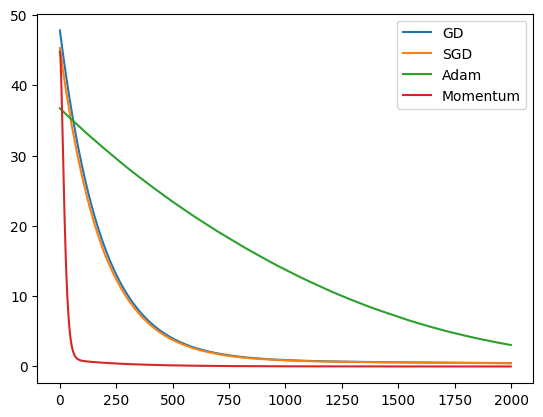
\includegraphics[width=0.9\linewidth]{lin_art.png}
    \caption{Линейная регрессия на искусственно сгенерированных данных}
    \label{lin_art}
  \end{subfigure}%
  \begin{subfigure}{.5\textwidth}
  \centering
    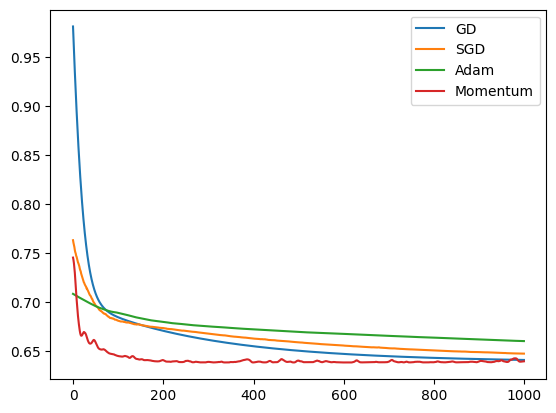
\includegraphics[width=0.9\linewidth]{log_art.png}
    \caption{Логистическая регрессия на искусственно сгенерированных данных}
    \label{log_art}
  \end{subfigure}
\end{figure}

\section*{Проверка на реальных данных}
\subsection*{Линейная регрессия}
В качестве набора данных для линейной регрессии используем \href{https://www.kaggle.com/datasets/yasserh/wine-quality-dataset}{Wine Quality Dataset}, где зависимым признаком является качество вина. 

На рисунке \ref{lin_real} представлены графики изменения функций потерь для различных вариантов градиентного спуска.

\begin{figure}[h]
    \centering
    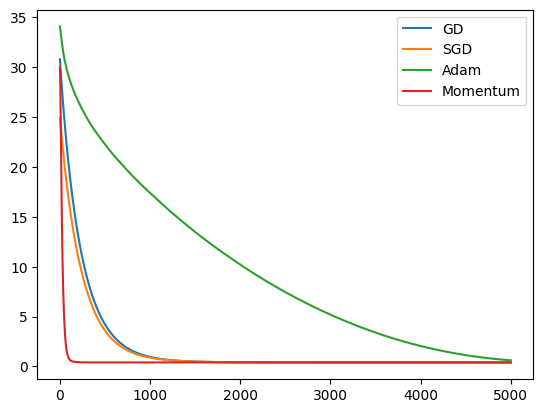
\includegraphics[width=0.5\linewidth]{lin_real.png}
    \caption{Линейная регрессия на реальных данных}
    \label{lin_real}
\end{figure}

Помимо применения реализованной модели, также была обучена и модель из библиотеки sklearn. Далее для всех моделей были рассчитаны метрики R-squared, Adjusted R-squared и Mean Squared Error. Полученные значения приведены в таблице \ref{lin_metrics}.

\begin{table}[h]
    \centering
    \begin{tabular}{c|c|c|c}
        \textbf{Модель}& \textbf{R-squared} & \textbf{Adjusted R-squared} & \textbf{MSE} \\\hline
         \textbf{GD}&0.391&0.363& 0.473\\
         \textbf{SGD}& 0.406&0.379& 0.461\\
         \textbf{Adam} & 0.079&0.037& 0.715\\
         \textbf{Momentum }& 0.404&0.377& 0.463\\
         \textbf{sklearn LR} & 0.4&0.373& 0.466\\
    \end{tabular}
    \caption{Значения метрик для линейных моделей на реальных данных}
    \label{lin_metrics}
\end{table}
\subsection*{Логистическая регрессия}
Для проверки логистической регрессии был использован \href{https://www.kaggle.com/datasets/mathchi/diabetes-data-set}{Diabetes Dataset}. На нём были обучены логистические модели с различными вариантами градиентного спуска. Сравнение функций потерь моделей представлено на рисунке \ref{log_real}. ROC-кривые для моделей 
показаны на рисунке \ref{log_real_roc}.

\begin{figure}[h]
  \begin{subfigure}{.5\textwidth}
  \centering
    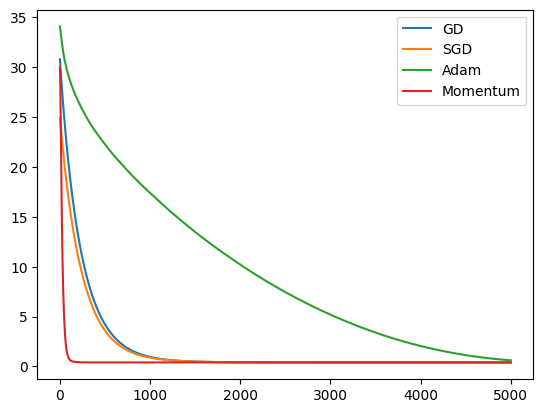
\includegraphics[width=0.9\linewidth]{lin_real.png}
    \caption{Функции потерь для логистической регрессии на реальных данных}
    \label{log_real}
  \end{subfigure}%
  \begin{subfigure}{.5\textwidth}
  \centering
    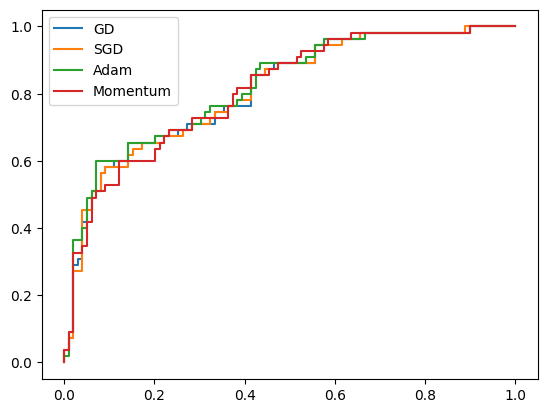
\includegraphics[width=0.9\linewidth]{log_real_roc.png}
    \caption{ROC-кривые для логистической регрессии на реальных данных}
    \label{log_real_roc}
  \end{subfigure}
\end{figure}

Помимо этого, для данных моделей и стандартной модели из библиотеки sklearn были измерены значения метрики AUC-ROC. Их значения приведены в таблице \ref{auc_roc}.

\begin{table}[h]
    \centering
    \begin{tabular}{c|c}
        \textbf{Модель} & \textbf{AUC-ROC} \\\hline
         GD&0.814\\
         SGD&0.812\\ 
         Adam&0.821\\ 
         Momentum&0.811\\ 
         sklearn&0.735\\ 
    \end{tabular}
    \caption{AUC-ROC для логистической регрессии на реальных данных}
    \label{auc_roc}
\end{table}
\end{document}